\documentclass[11pt,a4paper,slovak]{article}

\usepackage[utf8]{inputenc}
\usepackage[T1]{fontenc}
\usepackage[slovak]{babel}
\usepackage[sfdefault]{FiraSans}
\usepackage[margin=2.5cm]{geometry}
\usepackage{microtype}
\usepackage{cite}
\usepackage{hyperref}

\usepackage{graphicx}


\usepackage{url} 
\usepackage{hyperref}
\usepackage{tabularx}
\usepackage{changepage}
\usepackage{float}
\usepackage{xcolor, colortbl}
\usepackage{booktabs}


\definecolor{Gray}{rgb}{0.88,0.87,0.88}
\newcolumntype{a}{>{\columncolor{Gray}}c}
\newcolumntype{e}{>{\columncolor{Gray}}l}
\newcolumntype{f}{>{\columncolor{Gray}}r}
\newcolumntype{d}{>{\columncolor{Gray}}p{0.4\textwidth}}
\newcolumntype{z}{>{\columncolor{Gray}}X}

\newcommand{\thinline}{\arrayrulecolor{gray}\specialrule{0.2pt}{0pt}{0pt}\arrayrulecolor{black}}


\renewcommand{\arraystretch}{1.4}
\setlength{\extrarowheight}{2pt}



\hypersetup{
	colorlinks=true,
	linkcolor=black,
	citecolor=blue,
	urlcolor=black
}

\setlength{\parindent}{0pt}
\setlength{\parskip}{0.55em}
\setlength{\emergencystretch}{2em}

\pagestyle{headings}

\title{Prehľadový článok}
\author{Martina Bublincová\\
	Ján Danečko\\
	Andrej Thomas Dobrev\\
	Michal Furman\\[6pt]
    {\small Metódy inžinierskej práce}\\
	{\small Slovenská technická univerzita v Bratislave}\\
	{\small Fakulta informatiky a informačných technológií}
}
\date{\small 30. september 2026}

\begin{document}
\maketitle
\thispagestyle{empty}
\newpage

\section{Názov projektu}

Personalizovaný asistent sústredenia študentov

\section{Akronym}

PASS

\begin{quote}
``Use PASS to pass a test.''
\end{quote}

\section*{Abstrakt}
Projekt PASS sa zameriava na problém digitálneho vyrušovania pozornosti študentov počas učenia. Mobilné telefóny sú častým distraktorom nielen kvôli notifikáciám, ale aj vďaka spontánnemu otváraniu aplikácií.

Hlavným cieľom projektu je navrhnúť koncept mobilnej aplikácie určenej na zber, spracovanie a vizualizáciu údajov o rušení pozornosti počas učenia. Na základe identifikácie individuálnych vzorcov správania bude možné navrhnúť používateľovi vhodné metódy a cielené opatrenia pre zníženie vplyvu rušivých digitálnych stimulov a návykov.

Projekt bude zahŕňať analýzu existujúcich riešení a súčasnej situácie výskumu v oblasti digitálneho rozptyľovania, návrh na efektívne vyhodnocovanie zozbieraných údajov a ich vzťahu s reakciami používateľa. Na rozdiel od bežných nástrojov založených na plošnom blokovaní notifikácií bude aplikácia PASS založená na individuálnom správaní a reakcii na konkrétne podnety, pričom bude používateľ informovaný o podvedomej manipulácii s mobilným telefónom a vyhľadávaní rozptýlenia.

Navrhnutá aplikácia bude mať jednoduché používateľské rozhranie, s dvomi základnými maskami: Profil a Štúdium. Funkcia Štúdium aktivuje režim zberu dát a zapne reštrikcie podľa nastavení v sekcii Profil. Aplikácia zozbiera informácie o využívaní iných aplikácií, notifikáciách a reakciách používateľa. Po ukončení režimu Štúdium aplikácia uloží nazbierané údaje, spracuje ich a vyhodnotené informácie vráti do sekcie Profil, kde ich používateľ môže sledovať a rozhodovať o nasledujúcich opatreniach. Medzi ďalšie funkcionality budú patriť aj dlhodobé výsledky formou grafov, kalendár štúdia, body za nepretržitú sériu študijných relácií a časovače.

Výsledkom bude koncept mobilnej aplikácie na systematickú podporu sústredenia počas štúdia, pričom rozhodnutia o konkrétnych krokoch a obmedzeniach aplikácií a notifikácií ostane vždy konečným rozhodnutím používateľa.

\section{Úvod}

Častá kontrola mobilného telefónu, ako aj jeho dlhodobé používanie zvyšujú mentálne úsilie, čím narušujú proces učenia. \cite[p.~40]{Liao2026} Dôsledkom neregulovaného správania na základe prichádzajúcich upozornení sú dokázané zhoršené akademické výsledky študentov. \cite[str.~18:20]{Kim2021}

Motívom našej práce bol aj ďalší zaujímavý výskum, ktorý ukázal, že používanie smartfónu počas  vyučovacej hodiny, kde bol výskum realizovaný, nie je jednorazové správanie, ale proces, ktorý ovplyvňujú vonkajšie podnety aj vnútorný stav študenta. Častejšie používanie telefónu spôsobovali vonkajšie podnety, ako sú notifikácie, a tiež osobná pozornosť voči telefónu. Dlhšie používanie sa však objavilo aj bez vonkajších podnetov, a to vplyvom osobných návykov a pozornosti voči telefónu. Preto plošné odstránenie notifikácií samo o sebe nemusí vyrušovanie znížiť, ako sa všeobecne predpokladá. Na učenie mala väčší vplyv priemerná dĺžka jedného použitia telefónu než jeho frekvencia, takže je vhodné sledovať ich oddelene. \cite[str.~41, 42]{Liao2026}

Priestor pre implementáciu nášho riešenia sa teda otvára, pretože problém, ktorý sa doteraz mohol zdať vyriešený stíšením upozornení naberá po dôsledných výskumoch nový rozmer. Aj autori iného výskumu, citovaného v našej práci potvrdzujú, že ich výsledky ponúkajú nové poznatky pre návrh inteligentých systémov riadenia rozptýlenia v kontexte učenia. \cite[str.~18:20]{Kim2021}

Cieľom projektu PASS je navrhnúť mobilnú aplikáciu, ktorá bude monitorovať nielen prijaté notifikácie, ale predovšetkým reakcie používateľa a jeho následné digitálne správanie počas učenia. Na základe získaných údajov aplikácia identifikuje individuálne vzorce správania a navrhne personalizované opatrenia na obmedzenie digitálneho vyrušovania. O ich zavedení do nastavení zariadenia a aplikácií bude rozhodovať samotný používateľ. Cieľom projektu teda nie je iba blokovanie notifikácií počas učenia, ale predovšetkým personalizácia digitálneho prostredia podľa potrieb a návykov konkrétneho študenta.

\section{Súvisiace práce}

Digitálne zariadenia predstavujú počas učenia významný zdroj rozptýlenia, a tak môžu negatívne ovplyvňovať aj samotné výsledky učenia. Napríklad výskum Kima a kol. (r. 2021) ukázal, že spôsob, akým študenti reagovali na notifikácie mal priamy vplyv na ich študijné výsledky. Študenti, ktorí dokázali ignorovať upozornenia mali výsledky lepšie. Reakcie nasledované dlhšími reláciami používania sa ukázali ako škodlivé. Napriek tomu, že autori výskumu súhlasia s faktom, že smartfóny môžu byť užitočným nástrojom na štúdium, no zároveň upozorňujú, že notifikácie môžu byť spúšťačom ich nadmerného používania. \cite[str.~18:20]{Kim2021}

Výskum (Telypova a kol., 2025) sa zameral na to, ako sa ľudia pri práci rozptyľujú pri používaní viacerých zariadení. Autori zistili, že schopnosť udržať pozornosť pri jednej úlohe sa neustále skracuje. Dôležité pritom je, akým smerom prebieha prechod medzi činnosťami: prepnutie na aktivitu, ktorá podporuje prácu, sa líši od prepnutia na rušivú aktivitu. Na sústredenie vplývajú aj osobnostné črty, najmä svedomitosť, naliehavosť pri negatívnych emóciách a prívetivosť. Koncentráciu ďalej zhoršuje denná doba, stres a únava. Autori preto odporúčajú vytvárať systémy, ktoré rozpoznajú možné vyrušenie vopred, dokážu odložiť notifikácie a pritom ponechajú používateľovi kontrolu nad vlastným správaním. \cite[conclusion]{10.1145/3729176.3729198}

Pri monitorovaní skúmanej oblasti sme sa okrem samotného problému zamerali aj na analýzu existujúcich riešení zameraných na sústredenie. Napríklad Grover a kol. (2020) vo svojom výskume navrhli a vyhodnotili inteligentných agentov na podporu produktivity a sústredenia v pracovnom prostredí. Ich riešenie okrem plánovania úloh zahŕňalo aj monitorovanie vyrušení. Výsledky používateľskej štúdie poukázali na potenciál takýchto nástrojov pri podpore produktivity, pričom účastníci zároveň zdôraznili potrebu personalizovanejšieho plánovania a inteligentnejšieho monitorovania rozptýlení. \cite{10.1145/3377325.3377507} Napriek podobnému zameraniu sa však nástroj orientuje na podporu produktivity pracovníkov pri plnení úloh a nie na sústredenie študentov počas učenia. Efektivita prototypov bola založená najmä na upozorneniach na pracovnej ploche, ktoré pomáhali pracovníkom organizovať si pracovný deň, pričom ich prínos bol skúmaný v kancelárskom prostredí. \cite{10.1145/3377325.3377507}  My sa naopak nezameriavame na organizáciu pracovného rozvrhu, ale na monitorovanie digitálneho správania študentov počas učenia a prestávok. Naším cieľom je identifikovať konkrétne zdroje vyrušovania, ako sú notifikácie či spontánne otváranie aplikácií, a na základe získaných údajov poskytovať personalizované odporúčania.

\section{Návrh a fungovanie aplikácie}

Projekt PASS budeme realizovať formou mobilnej aplikácie, ktorá bude určená pre zariadenia s operačnými systémami Android a iOS. Jej hlavnou úlohou bude monitorovať digitálne správanie používateľa počas učenia a prestávok, vyhodnocovať získané údaje a na ich základe navrhovať individuálne opatrenia na zlepšenie sústredenia.

Aplikácia bude pozostávať z dvoch hlavných častí – Profil a Štúdium. V časti Štúdium používateľ spustí študijnú reláciu, počas ktorej bude prepínať medzi dvomi režimami: Štúdium a Prestávka. Počas oboch režimov bude aplikácia zaznamenávať používanie mobilného zariadenia, prijaté upozornenia a reakcie používateľa na ne. Dôležité je, že zhromažďovanie údajov sa nebude obmedzovať iba na čas učenia. Aplikácia bude sledovať aj priebeh prestávok, pretože ich účelom je regenerácia pozornosti a fyzický či psychický oddych, nie pokračovanie v digitálnej aktivite. Po ukončení študijnej relácie sa získané údaje spracujú a uložia do časti Profil. Používateľ tu bude môcť sledovať svoje digitálne návyky prostredníctvom grafov, štatistík a dlhodobých prehľadov. Na základe týchto informácií aplikácia identifikuje najčastejšie zdroje vyrušovania a navrhne používateľovi vhodné opatrenia. Ich zavedenie bude závisieť od jeho vlastného rozhodnutia.

\centering{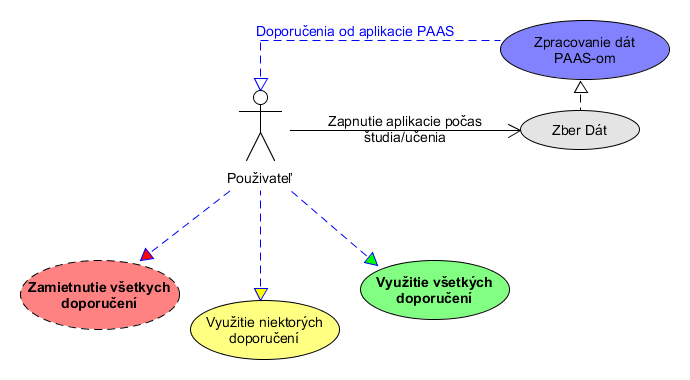
\includegraphics[width=0.7\textwidth]{diagramPNG.png}}

\section{Zber a analýza údajov}

Základom fungovania PASS bude zhromažďovanie údajov o digitálnom správaní používateľa, a to počas režimov Štúdium aj Prestávka. Aplikácia sa nebude zameriavať iba na samotný čas strávený v jednotlivých aplikáciách, ale predovšetkým na okolnosti ich používania a reakcie používateľa na digitálne podnety.

Medzi sledované údaje budú patriť prijaté upozornenia, ich počet a aplikácie, z ktorých pochádzajú. Rovnako aj reakcie na upozornenia, čas, ktorý uplynul od ich prijatia po reakciu, správanie po reakcii na upozornenie.

Keďže používanie digitálnych distraktorov sa nevyskytuje len vďaka notifikáciam, sledovať budeme aj samostatné otváranie aplikácií. Sú to prípady, keď používateľ otvorí inú aplikáciu bez toho, aby ho k tomu podnietilo prichádzajúce upozornenie.

Rátame aj s možnosťou, že študent pri učení využíva telefón aj na samotné štúdium. V tomto prípade budeme sledovať pracovné nástroje a aplikácie určené na štúdium vo vzťahu so sociálnymi sieťami a inými nežiaducimi aplikáciami.

Zaznamenávať budeme aj dlhodobé správanie. Budú to napríklad zmeny v používaní aplikácií a reakcie na upozornenia v priebehu viacerých dní a študijných relácií. Získané údaje sa následne spracujú do prehľadných štatistík a vizualizácií. Používateľ bude môcť sledovať napríklad pomer prijatých a otvorených upozornení, priemerný čas reakcie podľa jednotlivých aplikácií, rozdelenie času stráveného v aplikáciách či vývoj ich používania v priebehu viacerých dní.

Dôležitou súčasťou vyhodnocovania bude identifikácia individuálnych vzorcov správania. Aplikácia sa tak pokúsi rozpoznať, ktoré aplikácie používateľa vyrušujú najčastejšie, či reaguje na upozornenia okamžite, alebo či má tendenciu spontánne kontrolovať telefón aj bez konkrétneho podnetu. Zároveň bude možné sledovať, či používateľ počas prestávok skutočne oddychuje, alebo ich väčšinu trávi používaním mobilného zariadenia.

\section{Personalizácia a podpora sústredenia}

Hlavným prínosom PASS nebude automatické blokovanie aplikácií a upozornení, ale personalizácia digitálneho prostredia na základe skutočných návykov konkrétneho používateľa.

Na rozdiel od bežných režimov sústredenia, ktoré umožňujú najmä plošné vypnutie upozornení alebo časové obmedzenie používania aplikácií, PASS bude vychádzať z individuálneho správania študenta. Na základe zozbieraných údajov mu odporučí konkrétne opatrenia, napríklad vypnutie upozornení z aplikácií, ktoré ho najčastejšie vyrušujú, alebo ich úplné obmedzenie počas študijnej relácie.

Používateľ však bude mať vždy konečné rozhodnutie. Nie každé upozornenie je totiž zbytočné a nie každá aplikácia predstavuje počas učenia rušivý prvok. Niektorí študenti potrebujú byť dostupní kvôli práci, rodine, blízkym osobám alebo zdravotným pripomienkam. PASS preto nebude automaticky obmedzovať všetky aplikácie, ale umožní používateľovi vybrať si, ktoré odporúčania chce prijať a akým spôsobom si chce zariadenie prispôsobiť.

Aplikácia sa bude snažiť zlepšovať aj kvalitu prestávok. Ich účelom nie je iba prerušenie učenia, ale predovšetkým odpočinok a regenerácia pozornosti. PASS preto bude používateľa motivovať, aby prestávky netrávil nekonečným prezeraním sociálnych sietí a iných aplikácií, ale venoval ich aktivitám podporujúcim fyzickú a psychickú pohodu. Môže ísť napríklad o pitie vody, krátku prechádzku, pohyb, oddych alebo uspokojenie základných fyzických potrieb. Používateľ si zároveň bude môcť prispôsobiť dĺžku prestávok, nastavovať časové obmedzenia a určiť minimálny čas učenia pred ďalšou prestávkou.

Dlhodobým cieľom je, aby používateľ postupne získal lepší prehľad o vlastných digitálnych návykoch, naučil sa rozpoznávať situácie, v ktorých stráca pozornosť, a dokázal svoje správanie vedome regulovať. PASS teda nechce používateľovi telefón odobrať ani mu zakázať jeho používanie. Chce mu pomôcť vytvoriť také digitálne prostredie, v ktorom bude môcť zostať dostupný pre dôležité informácie, no zároveň nebude zbytočne vystavovaný podnetom, ktoré narúšajú jeho sústredenie.

\section{Implementácia a experiment}


\begin{table}[H]
\centering
\begin{adjustwidth}{-0.5cm}{-0.5cm}
\begin{tabularx}{\linewidth}{|l|l|X|}
\hline
\multicolumn{1}{|e|}{VV-D} & \multicolumn{2}{|f|}{Harmonogram projektu} \\ \hline
\multicolumn{1}{|e|}{Začiatok etapy} & \multicolumn{1}{|e|}{Koniec etapy} & \multicolumn{1}{|e|}{Názov etapy}\\ \hline
1.1.2027  & 31.1.2027 & Vývoj prototypu aplikácie \\ \hline
1.2.2027 & 14.2.2027 & 1. vlna testovania prototypu \\ \hline
14.2.2027 & 14.3.2027 & Zlepšenie prototypu \\ \hline
15.3.2027 & 28.3.2027 & 2. vlna testovania prototypu \\ \hline
28.3.2027 & 4.4.2027 & Záverečné vylepšenia a zhotovenie vysledkov testovania \\ \hline

\end{tabularx}
\end{adjustwidth}
\end{table}


\section{Výsledky}

Podľa čoho zistíme či projekt funguje?

Aké výsledky očakávame, ako ich zhodnotíme?

\section{Záver a možné rozšírenia projektu}

Čo by sme projetkom zistili, dosiahli?

Ako by sa dal projekt ďalej rozšíriť a čo by prinášal?

\bibliographystyle{unsrt}
\bibliography{references}

\end{document}
